% Chapter 2
\chapter{Background} % Main chapter title
%\epigraph{A fancy quote.}{Me}

\label{Background} % For referencing the chapter elsewhere, use \ref{Chapter2} 
\lhead{Chapter 2. \emph{Background}} % Main chapter title % This is for the header on each page - perhaps a shortened title

In this chapter we provide background knowledge required to understand the rest of the document. We start by presenting, in the first section, a possible definition of the main concept of this work, \textit{relevance}. In the two last sections we give a quick introduction to some basic concepts used in the NLP and ML fields.

%----------------------------------------------------------------------------------------
\section{Definition of \textit{Relevance}}

As \textit{relevance} became a subject of research among the years, many tried to address its definition. For instance, Saracevic~\citep{Saracevic1996RelevanceReconsidered,Saracevic2007RelevanceReview} points out its nature and manifestations, such as:

\begin{itemize}
	\item \textbf{System or algorithmic relevance} - Relation between a certain query and the retrieved objects obtained through some algorithm or procedure. Relevance is then inferred through a comparison of the results. Search systems where a user needs to input a search query and get quality results related to the search term are good examples. 
    \item \textbf{Topical or subject relevance} - Relation between the topic or subject of a query and the topic or subject of the retrieved objects. Aboutness, which is a closely related concept to relevance, deals with the organization and hierarchy of information and can be used to provide results that more likely to be related to the topic of the search term. An user searching for the concept ``informatics'', will get results that are at least related to the same field of study of the concept, i.e., the same topic. 
    \item \textbf{Cognitive relevance or pertinence} - Relation between the desired knowledge by the user for a specific query and the actual retrieved objects. Cognitive relevance is inferred through the informativeness, novelty and information quality of the retrieved objects. As an example, a user might be searching for the programming language 'R' and obtain results about the alphabet letter, which was not what he intended.
    \item \textbf{Situational relevance or utility} - Relation between the problem-at-hand and the objects retrieved. To measure this relevance, criteria like usefulness may be used. For example, an user might be searching for a solution on how to fix a device, and although he does not know exactly what results he is expecting, he can measure it by its usefulness, i.e., if it helped solving the problem. 
    \item \textbf{Motivational or affective relevance} - Relation between the intents and goals of a user and the retrieved objects. To measure this kind of relevance, metrics like satisfaction, success or accomplishment may be used. In this case there is no user input and thus is more related to the scope of this work which evaluates if a particular content is somehow relevant.
\end{itemize}

%Nowadays, there are two well-known measures to evaluate the performance of an IR system. They are precision and recall and they measure the proportion of relevant documents retrieved from a search and the proportion of relevant documents that are retrieved. In fact, recall was once called \textit{relevance} but was renamed later to avoid confusion \citep{Kent1955PrecisionRecall}.

Information quality is closely related to \textit{relevance}, as it measures the value that the information provides to the user. Since the Web is full of unstructured and inconsistent data, it is important to find ways to measure the quality or \textit{relevance} of the information for a specific problem faced by a user. Saracevic \citep{Saracevic2012QualityInformation} showed possible measurements for assessing the quality of information, such as the intrinsic characteristics of the text, the context of the information, its representation and access:

\begin{itemize}
	\item \textbf{Authority} and \textbf{verifiability}: text should be elaborated by a credible and respected entity;
    \item \textbf{Objective} and \textbf{reliable}: the information conveyed should avoid individual biases and be trustworthy;
    \item \textbf{Relevant}, \textbf{appropriate} and \textbf{comprehensive}: the context of the information should be related to the topic of the problem-at-hand and complete;
    \item \textbf{Timeliness}: well-timed information related to the task is typically useful;
    \item \textbf{Organization}, \textbf{suitability} and \textbf{conciseness}: express coherent and logical thinking, consistency across different sources, and representation in a simple and compact manner;
    \item \textbf{Availability}, \textbf{convenience},  \textbf{security} and \textbf{integrity}: easy to access, easy to use, good protection politics, and good ethics.
\end{itemize}

%In terms of the intrinsic characteristics of the text, it should be elaborated by credible and respected entities (authority) and also be verifiable (verifiability). The information should avoid individual biases, be faithful to the truth (objectivity) and trustworthy (reliability).
%The context of the information should be related to the topic of the problem-at-hand and be appropriate and complete (relevance, appropriateness, comprehensiveness). Besides, well-timed information related to the task is also useful (timeliness). In terms of representation, usual characteristics like coherent and logical thinking (organization), simple and clear understanding (suitability), consistency across different sources and representation in a simple and compact manner (conciseness) are good metrics to achieve. Finally, the information should also be easy to access (availability), easy to use (convenience), have good protection politics (security) and follow good ethics (integrity).\\
Quality and \textit{relevance} measurement of information is usually a task performed by humans.
Yet, if accurate enough, computer-assisted classification is obviously very useful for the end user, which will save time otherwise spent on filtering irrelevant information, and lead to a better experience overall. The scope of this work involves automating this process by classifying instances as relevant or irrelevant.

\subsection{Relevance from an Information Retrieval Perspective}

To improve efficiency in traditional Information Retrieval, strings of text are mapped to simpler representations. The process of mapping the contents of a document into a compact representation that can be later used is sometimes called \textit{indexing}. A very common representation is the vector space model. In this model each document is represented by a vector of words. Usually there is more than one document, therefore a term $\times$ document matrix $M$ is usually used, with each entry representing the importance, relevance or weight of a given word in a certain document. Since the number of words can be huge, a common problem with this kind of representation is the dimensionality of the feature space. %However there are ways to minimize this problem such as dimensionality reduction techniques. 
From the point of view of natural language, this brings questions such as identifying the meaningful units of text (lexical semantics) and the rules for combination (compositional semantics). 
Each cell of the term $\times$ document matrix measures the term contribution for the classification task. In order to determine the value of these weights, different approaches might be followed, typically one of the following\citep{Sebastiani2002MLTC, Yadav2015TextFiltration,Patra2013SurveyTCAlgorithms}:
\begin{itemize}
	\item \textbf{Boolean weighting} - Each cell either has the value 1, if the word is present in the document, or 0, if it not. 
    \item \textbf{Word frequency weighting} - Word frequencies are used as the weights.
    \item \textbf{Term Frequency–Inverse Document Frequency (TF-IDF)} - This technique takes into account the fact that a word might appear in other documents, decreasing its weight when there are occurrences of the word in other documents.
    \begin{figure}[H]
      \centering
    	\[ tfidf(t_k,dj)) = \#(t_k,d_j) \cdot \log (\frac{N}{n_k}) \]
      \end{figure}
      where \#$(t_k,dj)$ is the number of times the term t$_k$ appears in document $d_j$, N is total number of documents and $n_k$ is the number of documents where the term $t_k$ appears. This follows the assumption that when a term occurs many times in a text it contributes to characterize this document but the more often it appears in other documents, the less it discriminates. It is also important to note that TF$\times$IDF does not account for the order of the words in the text, ignoring their syntactic role, i.e., only the lexical semantics and not compositional semantics. 
      \item \textbf{Normalized TF-IDF} - In order to normalize the vectors, length normalization is usually used. 
      \begin{figure}[H]
      \centering
    	\[ tfidf(t_k,dj)) = \frac{tfid(t_k,d_j)}{\sqrt{\sum_{1}^{N}[\#(t_k,d_j)\cdot \log (\frac{N}{n_j})]^2}} \]
      \end{figure}
      This is the most common used weighting method. It considers that the documents might have different lengths.
\end{itemize}

These indexing techniques are useful to determine the most relevant terms.

%  For example, Google uses the classic PageRank method to rank web pages according to their relevance by counting incoming links and outgoing links of a given page, weighting them differently and normalizing them by the total number of links, creating a probability distribution of the relevance of all the web pages, answering the intuitive question of what is the probability of a random user browsing the web ending up in a given page  \citep{PageBrinPageRank1999,BrinPageGoogleAnatomy2012}.
Another classic reference in sorting documents by its relevance is the PageRank algorithm, used by Google. PageRank uses the link structure of the web documents, i.e, a directed graph where each node represents a web document and each edge is an outgoing or incoming link from a given page (node), to produce a probability distribution representing the likelihood of a random person ending up on a particular page by randomly surfing through the web. Using this structure, the PageRank (\textit{PR}) of each document \textit{d}, can be obtained as follows\citep{PageBrinPageRank1999,BrinPageGoogleAnatomy2012}: 

\[\displaystyle PR(d) :=   \frac{1-\alpha}{N}  + \alpha \sum_{p\in O(d)} \frac{PR(p)}{L(p)}\]

where $N$ is the total number of documents, $L(p)$ is the number of outgoing links from the page $p$ belonging to the set of documents $O$ that link to the document $d$. The constant $\alpha$ represents the probability that an hypothetical user does not reach the target page while surfing. Each page contributes equally to each of the outgoing links. Therefore, if a document has many incoming links, its ranking rises. 

These are good models to define the relevance of documents. Although the concept of relevance is well-understood in the Information Retrieval field, it becomes challenging to define when we are in the presence of only raw text and are restricted to textual features such as features coming from the NLP field, where this work is included. It also becomes a problem when we have no direct information from the user such as search queries from where the terms might be extracted and used to retrieve the most related information. In fact, in Information Retrieval there is a strong relationship with the information given by the user, since the retrieved information has to be strongly related to the user input and in our study problem we simply do not have that information. 

\section{Natural Language Processing}
Humans communicate in natural language. In fact, this is a complex feature that sets us apart from the other species. NLP has been a topic of study since the 50s, rising from the intersection Artificial Intelligence (AI) and linguistics. According to Alan Turing (Turing, 1950), a fully intelligent system would have to possess natural language processing capabilities, among others, in order to communicate. ELIZA (Weizembaum, 1966), a simulation of a Rogerian psychotherapist, is often cited as one of the first autonomous system with NLP capabilities. Since then, there have been many attempts at creating artificial bots up until recently with the rise of intelligent assistants such as Google Now\footnote{https://www.google.com/search/about/learn-more/now}, Cortana\footnote{https://support.microsoft.com/en-us/help/17214/windows-10-what-is} or Siri\footnote{http://www.apple.com/ios/siri}. During a long period, NLP strongly followed symbolic, hand-crafted rules approaches, backed by the Chomsky theoretical works. However, due to the ambiguous nature of the natural language, these techniques often created ambiguous results, meaning that there were more than one way to interpret the language. In fact, one of the aspects that make NLP hard is the ambiguity present in natural language. With the rise of machine learning techniques, the paradigm shifted to Statistical Processing, relying more on probabilities, with varied success. Besides, large annotated corpora were used to train machine learning algorithms \citep{nadkarni2011NLPIntro}.\\
Usually computers either try to understand the language in order to communicate or to extract information from it. In this work, we are interested in the second case. Since the Web is composed mostly of text, artificial models need to understand the written languages in order to extract new knowledge and perform diverse tasks such as information searching, machine translation or, in our case, text classification. \\
We e will use concepts and techniques from the domain of NLP to extract features from text. Feature extraction is an important part of this work and affects directly the performance of the classifier. This section provides a revision of important concepts and techniques of this field that are useful in the feature extraction process. 

\subsection{Language Knowledge Levels}
In a typical dialogue there are different types of knowledge involved. From the moment that a person or system recognizes speech until the moment where it creates new dialogue, there is a set of intermediate steps a person or system need to know.\\
The following list represents the knowledge levels involved in a typical conversation \citep{Jurafsky2009SLP}:
\begin{itemize}
	\item \textbf{Phonetics and Phonology} - The participants involved in a conversation need to know how to pronounce words and how to recognize them from speech.
    \item \textbf{Morphology} - In order to know how to form words, knowledge about the creation, characterization and analysis is required. Usually, tasks such as lexical analysis are performed in this step, by identifying stems, roots or part-of-speech.
    \item \textbf{Syntax} - In order to create phrases and glue together words, structural knowledge such as the relationships between words is required. Usually, tasks such as syntactic analysis are performed in this step. This includes identifying syntactic dependencies between words, their syntactic categories or syntagmas.
    \item \textbf{Semantics} - This step is related to the meaning of single words (lexical semantics) and also the meaning of grouped words (compositional semantics). Semantic analysis is usually performed in this step. Since a word might have more than one meaning, this disambiguation is solved in this phase.
    \item \textbf{Pragmatics} - Pragmatics relates to the relationships between the meaning and the context. That is, depending on the context, the real intentions and goals of a user might be expressed in nonexplicit ways.
    \item \textbf{Discourse} - This level relates to the relationships between different parts of a text. Thus, this task usually involves determining to which previous parts of the discourse some words, such as demonstratives or pronouns,  are referring to.
\end{itemize}

Usually these levels are related to each other. NLP is a vast research area. We can list four subareas of study: Speech Recognition, Speech Synthesis, Natural Language Generation and Natural Language Understanding. In our case, we are interested in the last one, since we need to have some understanding of the language in order to extract features from it. 

One the main problems in Natural Language is ambiguity. Ambiguity arises when there are multiple interpretations or meanings and it affects all levels mentioned before. It can occur at the word level (lexical ambiguity), at the the phrase level (syntactic ambiguity), it can depend on the context (pragmatic ambiguity) or even at the discourse level \citep{Jurafsky2009SLP}. There are other issues that make it hard, such as non-standard English (or other languages), present in social networks feeds. Examples of this are unusual spelling of words, hashtags, among others. Another problem is expressions that are specific to the language and do not have a direct meaning such as ``get cold feet'' or ``lose face''.  In terms of language technologies, some of them are almost solved such as spam detection, Part-of-Speech (hereafter, POS) tagging or Name Entity Recognition (hereafter, NER). Other tasks such as sentiment analysis, coreference resolution, word sense disambiguation, parsing, machine translation and information extraction are making good progress. However, problems such as question answering, paraphrasing, summarization and dialog are still really hard to solve \citep{Jurafsky2009SLP}. 
    




\subsection{Issues in Social Media Text}

In academic, official or business contexts, written documents typically use formal language.
This means that syntactic rules and linguistic conventions are strictly followed.
On the other hand, although typically used orally, informal language has become frequent in written short messages or posts in social networks, such as Facebook or Twitter.
In opposition to news websites, where posts are more elaborated, complex and with a higher degree of correctness, in text posted in social networks, it is common to find shorter and simpler sentences that tend to break some linguistic conventions (e.g. proper nouns are not always capitalized, or punctuation is not used properly), make an intensive use of abbreviations, and where slang and spelling mistakes are common.
For instance, in informal English, it is common to use colloquial expressions (e.g.~``look blue'', ``go bananas'', ``funny wagon''), contractions (e.g.~``ain’t'', ``gonna'', ``wanna'', ``y’all''), clichés~(e.g.~``An oldie, but a goodie'', ``And they all lived happily ever after''), slang~(e.g.~``gobsmacked'', ``knackered''), abbreviations~(e.g.~``lol'', ``rofl'', ``ty'', ``afaik'', ``asap'', ``diy'', ``rsvp''); the first and the second person, imperative~(e.g.~``Do it!'') and usually active voices, in addition to the third person and the passive voice, which are generally only present in formal text.
Informal language poses an additional challenge for NLP tools, most of which developed with formal text on mind and significantly dependent on the quality of the written text.

Given the huge amounts of data transmitted everyday in social networks, the challenge of processing messages written in informal language has received much attention in the later years.
In fact, similarly to well-known NLP shared tasks based on corpora written in formal language, including the CoNLL-2000, 2002 or 2003 shared evaluation tasks\citep{TjongCoNLL2003}, tasks using informal text have also been organized, including, for instance, the Making Sense of Microposts Workshop~(MSM~2013)\footnote{\url{http://microposts2016.seas.upenn.edu}} or tasks included in the SemEval workshops~(e.g.~Sentiment Analysis from Twitter~\citep{rosenthal2015SemEval}).


\subsection{Common NLP-related Tasks} 
\label{nlp_tasks}
NLP is a vast area with many subproblems. Here we list concepts that might be relevant for this work, i.e., potential tasks that can laid the groundwork for the feature extraction process. We can also divide these tasks in low-level tasks and high-level tasks that are usually built on top of low-level tasks \citep{nadkarni2011NLPIntro}. We list some of the most popular task applied to the phrase ``Jay visited back home and gazed upon a brown fox and quail.'':
\begin{itemize}
		\item \textbf{Word Tokenization} - Tokenization is usually the first step in NLP pipelines. It is the process of breaking down sentences into words, identifying individual tokens such as words or punctuation signals. Although this seems a relatively easy task, it has some issues because some words may rise doubts on how they should be tokenized, such as words with apostrophes, or with mixed symbols. For above example would become ``Jay$|$visited$|$back$|$ home$|$and$|$gazed$|$upon$|$a$|$brown$|$fox$|$and$|$quail$|$.$|$'' 
        \item \textbf{Word Normalization} - Text normalization is a frequent pre-processing task in NLP applications. It usually involves transforming the word tokens into their simpler forms. In order to achieve this, tasks such as case folding (converting letters to lower case), lemmatization (reduce the variant forms such as inflections and derivations to their original base form) or stemming (extraction of the root of the word) methods are employed. Usually morphology analysis plays an important role in this task. As an example, the previous phrase lemmatized would become ``Jay visit back home and gaze upon a brown fox and quail . '' or ``jay visit back hom and gaz upon a brown fox and quail .'' when stemmed.  
        %\item \textbf{Collocation Finding} - Collocations are groups of two or more words that usually go together. Methods based on frequencies are usually employed to find them.
        \item \textbf{Sentence Segmentation} - This task detects sentence boundaries and segments out sentences from text. Again the ambiguity of signs such as ``.'' makes this task more difficult that it may seem at first, since they may belong to abbreviations, numbers and not really an end of phrase. 
        \item \textbf{N-grams} - N-grams are sequence of \textit{n} contiguous words retrieved from a text. They are very useful to build language models, i.e, models where the probabilities of sequence of words are computed allowing for example, to predict the next word in a sequence, machine translation, spell correction, among others. Other useful application of n-grams is classification, i.e., an unigram model of a text, also called bag-of-words. The bag-of-words model, along with the word counts may be used as a vector of feature/value pairs for classification tasks. It is important to note that with an unigram model, the notion of order is lost. High order n-grams may be used to keep some order. For example, the bigrams from the above phrase would be: \{Jay visited, visited back, back home, home and, and gazed, gazed upon, upon a, a brown, brown fox, fox and, and quail\}.        
        A problem with this model is that the feature vector is very large and sparse, since for very small messages, most n-gram counts will be zero. If gaps between words are allowed, we called them skip grams. Skip grams are a generalization of n-grams since they include sequence of words that are separated in the original text by some distance.  
        \item \textbf{Part-of-speech Tagging} - The objective of the POS tagging is to determine the correct part-of-speech class for each token in a sentence, according to a specific tagset. In this work, the tags of the Penn Treebank Project \citep{MitchellPennTreebank1993}, popular among the NLP community, are used. The example phrase would then become: Jay$|$NNP(Proper noun, singular) visited$|$VBD(Verb, past tense) back$|$RB(Adverb) home$|$NN(Noun, singular) and$|$CC(Coordinating conjunction) gazed$|$VBN(Verb, past participle) upon$|$IN(Preposition) a$|$DT(Determiner)\\ brown$|$JJ(Adjective) fox$|$NN(Noun, singular) and$|$CC(Coordinating conjunction) quail$|$NN(Noun, singular) .$|$.
        \item \textbf{Shallow Parsing} - Chunking, also known as shallow parsing, is a lighter syntactic parsing task. The main purpose is to identify the constituents groups in which the words are organized, such as noun phrases (NP), verb phrases (VP) or prepositional phrases (PP). Glued together, these chunks form the entire sentence. They may also be nested inside each other forming a nested structure, such as trees, where each leaf is a word, the previous node is the corresponding POS tag and the head of the tree is the chunk type. The example phrase would become: Jay$|$NP$|$Noun-phrase
visited$|$VP$|$Verb-phrase back$|$O$|$Out-of-chunk home$|$NP$|$Noun-phrase and$|$O$|$Out-of-chunk gazed$|$VP$|$Verb-phrase\\
upon$|$PP$|$Prepositional-phrase a$|$NP$|$Noun-phrase brown$|$NP$|$Noun-phrase\\
fox$|$NP$|$Noun-phrase and$|$O$|$Out-of-chunk quail$|$NP$|$Noun-phrase
		\item \textbf{Name Entity Recognition/Classification} - As the name implies, Name Entity Recognition deals with the identification of certain types of entities in a text and may go further classifying them into one of given categories, typically PERson, LOCations, ORGanizations, all proper nouns, and sometimes others, such as dates. Usually this task is also useful to link mentions in the text to a specific entity. This usually involves other sub-problems such as Name Entity Disambiguation (NED), where an entity is fully specified and reference resolutions where mentions are linked to the original named entities. Although initials are a good indicator of potential entities, in social media text this task is harder since users do not always follow this rule, which complicates the process. In the example above, ``Jay'' would be identified as a Person.
        \item \textbf{Sentiment Analysis} - Sentiment is a classification task where each piece of text is classified according to their perceived sentiment, opinion or subjectivity. The complexity of this task may range from simple positive/negative labeling to a a set of ranking categories or even detecting complex attributes such as the source of such sentiment, the target and the type of sentiment (love, hate, positive, negative, neutral, etc). In classification tasks it is common to make extensive use of sentiment lexicons, i.e., a set of words labeled according to a certain type of sentiment, attitude, opinion, mood, etc.
        \item \textbf{Edit Distance} -The string edit distance or Levenshtein distance, is a distance metric between two strings equal to the minimum number of edits required to transform one string into another.
        %\item \textbf{Information Extraction} - Information Extraction is the task of extracting knowledge from unstructured data such as text and representing it in a structured way. It is very useful to organize information such as facts, events or relationships. A common used structure is a relation triple such as (Object1, Object2, Property). This knowledge base makes it easier for algorithms to understand the data and work on it.
		%\item \textbf{Relation Extraction} - This task is similar to information extraction but focus on the identification of relationships between different entities.
        %\item \textbf{Dependency Parsing} - A dependency structure allows to see the dependency between words, usually represented by directed edges, starting in a word and pointing to the word on which depends. This structure is useful to understand, in a graphical way, textual relations, such as who did what, when and where and how. 
        %\item \textbf{Coreference Resolution} - Coreference resolution tries to find and link every entity to its mentions in a text. It is an useful task for extract information from text.    
       % \item \textbf{Semantic Analysis} - Semantical Analysis is the step where the meaning of words is represented. In terms of lexical semantics, each lemma (noninflected form of a word) may have one or more word senses associated and may also be related to other lemmas though lexical relations such as synonymy, hypernym, meronym among many others. This information about the meaning of words and their relations can be structured in lexical knowledge databases such as the popular \href{https://wordnet.princeton.edu}{WordNet}\citep{miller1995wordnet}. An example are the synsets that group together words with the same sense. The knowledge database also groups the words under different categories such as nouns, verbs, adjectives or adverbs. Word Sense Disambiguation is a common application that makes use of this information.
        \item \textbf{Latent Dirichlet Allocation (LDA)} - Latent Dirichlet Allocation is a probabilistic model of a corpus,  where each document is represented by an explicit probabilistic distribution of latent topics (unobserved) and each topic is defined as a distribution over words. It is a process of discovering the topics that each document (set of words) in a corpus (set of documents) contains. LDA assumes that a given corpus was produced by a generative process and then tries to classify each document with a set of topics that, according to that model, were likely to have generated them. The generative process can be described as follows\citep{Blei2003latentdirichlet}:

\begin{algorithmic}
	\For{document $d$ in corpus $D$}  
    \State Choose the number of words $N \sim P(\xi)$ the document $d$ will have
    \State Choose a topic mixture $\theta_d \sim Dir(\alpha)$ for the document $d$
    \For{word $w_d$ in document $d$}
    	\State Pick a topic for the word $z_w \sim Multinomial(\theta_d)$
        \State Use the topic $z_w$ to generate the word from $p(w_d | z_w,\beta)$
    \EndFor
    \EndFor
\end{algorithmic}

The number of words $N$ is usually generated from a Poisson distribution $P(\xi)$, the topic mixture from a Dirichlet $Dir(\alpha)$ distribution, the topic of a word according to a Multinomial obtained from the topic mixture $\theta_d$ and the word itself $w_d$ according to the probability distribution of the chosen topic $z_w$.
  
\end{itemize}

These tasks give us a better understanding of the language and allows us to analyze it and extract useful information that we can use as features for a predictive model. In our work, we used tasks such as n-grams, part-of-speech tagging, chunking, name entity recognition, sentiment analysis and latent dirichlet allocation in order to extract features and establish the groundwork for the classification pipeline. 

\section{Machine Learning and Text Classification}

The problem of Text Classification is to decide which of a predefined set of classes or categories, a piece of text belongs to. Example applications of this nature are language identification, sentimental analysis, opinion detection, spam detection, among many others.\\ %A common characteristic of text is the high dimensionality of the feature space. If we consider a simple model where each word is as a feature, then the number of possible terms is very vast.
We usually describe the \textbf{objects} that we wish to recognize by a set of variables called \textbf{features}, consisting of information that we extract from the study objects. In the case of text classification, our study object is the text itself and we extract information using, for example, tasks presented in section \ref{nlp_tasks}.
Such features are then collected in vectors of \textbf{dimension $d$}, called \textbf{feature vectors}, usually denoted by $x$. They represent points in a $d$ dimensional space, called \textbf{feature space}. Each point belongs to a class, usually denoted by $w$ and the combination of the feature vectors and their corresponding class are called \textbf{patterns}. If we only have two target classes, as in this work (relevant or irrelevant), we are in the presence of a \textbf{binary classification} problem. 

\begin{figure}[htp]
	\centering
	\resizebox{\textwidth}{!}{
  	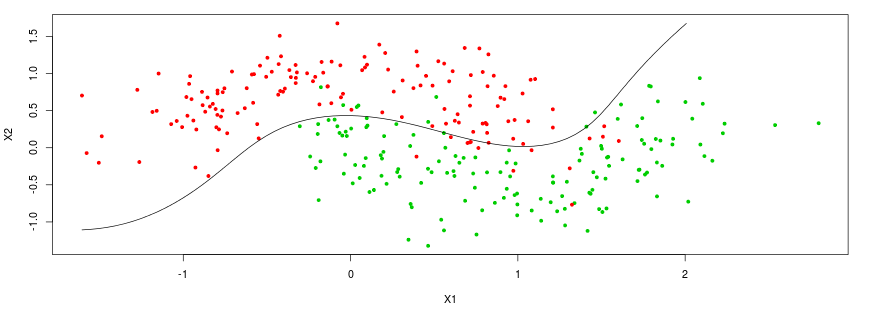
\includegraphics{./Figures/ML/decision_boundary}
     }
	\caption[Two class hypothetical example with non linear decision boundary]{Two class hypothetical example with non linear decision boundary}
	\label{fig:2-class-problem}
\end{figure}

Classification problems may be trivial for humans but are usually quite challenging for automated systems, since we need to deal with a lot of issues such as finding a reasonable number of distinguishing features good enough for classification, that are able to separate the target classes, or finding models that have good generalization capabilities (perform well on unseen data), avoiding overfitting of the model to the training data. Figure \ref{fig:2-class-problem} shows an hypothetical problem with two classes and two features. The main goal is then to find the best decision boundary that results in the best generalization on testing data. 

\begin{figure}[htp]
	\centering
	\resizebox{\textwidth}{!}{
  	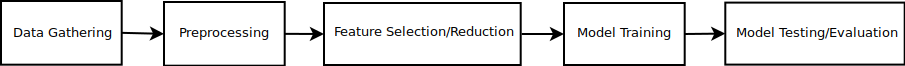
\includegraphics{./Figures/ML/ml-pipeline}
     }
	\caption[Typical pipeline of a machine learning application]{Typical pipeline of a machine learning application}
	\label{fig:ml-pipeline}
\end{figure}
 
Figure \ref{fig:ml-pipeline} shows the workflow of a typical machine learning application. Usually text classification involves steps such as data gathering, preprocessing, feature selection/reduction, training,testing and the final evaluation. The main goal is to assign, with the best accuracy possible, new labels to new documents. 

%Besides, text classification tasks can be divided between single-label or multi-label classification tasks and category-pivoted or document-pivoted text classification. When only one category is to be assigned to documents, it is called single-label classification, otherwise, if multiple labeling is allowed for a single document, it is a multi-label classification. In the case of document-pivoted classification, the goal is to assign one or more categories to a document. On the other hand, in category-pivoted classification the goal is to find all the documents that belong to a category. The former case is more common. This distinction because the set of classes and documents are not always available from the start, i.e, they may be added in different moments in time \citep{Niharika2012TC}. In this work, we are interested in single-classification, document-pivoted tasks.
\subsection{Data Gathering}
The first step is to collect the training and testing data such as sufficient and representative data. This usually implies tasks such as \citep{Gama2015DataMining}:
\begin{itemize}

	\item \textbf{Data Integration} - The initial data might come from different sources, with different formats or duplicated data. This step is important to create a single repository of data. 
    \item \textbf{Data Balancing} - As is often the case with real data, the data is usually not uniformly distributed across the different classes. Consequently, the trained models tend to predict new data with the majority class. Techniques to artificially balance the data might be employed here, such as reducing (Undersampling) / increasing (Oversampling) the number of instances from the majority /minority classes. Another alternative might be performing a stratified sampling in order to keep a significant number of instances in each class. Neighbor-based approaches \citep{mani2003knn,laurikkala2001improving} or synthesization of new examples \citep{chawla2002smote} are popular techniques used in this stage.
    \item \textbf{Cleaning} - The quality of the data is important. Sometimes the data will have missing attributes or useless values. However, redundant or noisy data are important issues to be addressed, such as instances with very similar feature values, attributes easily deducted from others or outliers.
\end{itemize}

Most of these steps were performed by the research team responsible for the data collection. Although, in this work some tasks such as removal of useless data and aggregation of duplicates with different labels were needed.  

\subsection{Preprocessing}
Some learning algorithms do not deal with certain types of data. In order to be able to use them, the type of the attributes might be transformed to another suitable type. For example converting symbolic features to equivalent numeric features, or the other way around. \\ Another important issue to consider is the normalization of the data, such as converting different attributes to the same scale, avoiding the dominance of some attributes and decreasing the dispersion of the data. Some example of used techniques are shown next:

\begin{itemize}
\item \textbf{Standardization} - Standardization transforms each feature by removing their mean and diving non-constant features by their standard deviation, obtaining data normally distributed with zero mean and unit variance ($\rho_{x_{std}}=0$,$\sigma_{x_{std}}=1$)
\[x_{std} = \frac{x - \rho _{X}}{\sigma _{X}}\]
\item \textbf{Normalization} - Normalization involves scaling samples/features vectors to have unit norm, usually achieved by diving by the euclidean norm of the vector.
\[x_{norm} = \frac{x }{\sqrt{\sum_i{x_{i}}^{2}}} \]
\item \textbf{Scaling} - Scaling transform the features to lie between a minimum and a maximum value. Typical ranges are [0,1] or [-1,1]. 
\[x_{[0,1]} = \frac{x - min _{x}}{max _{x} - min _{x}}\]
\end{itemize}

\subsection{Feature Selection}
Feature selection usually involves selecting a subset of the original set of features that provide the biggest discriminatory power, i.e., are able to provide the best separation between classes, result in the best performance of the classifier when trained and avoid the curse of dimensionality. In fact, it has been said in the literature that exists a critical feature dimension from where the performance degrades rapidily \citep{Ribeiro2015CFD}. Feature selection helps in removing irrelevant and redundant features and is usually divided into filter methods, where a subset of features is selected, without considering the predictive model and wrapper methods which use the classifier to rank and choose the best feature set. This step, in conjunction with feature reduction, is likely to be one of the most important steps in the pipeline. The following list shows common techniques employed in feature selection:

%\textbf{Filter Selection Methods}:
\begin{itemize}
	\item \textbf{Information Gain} - Information gain ranks each attribute by its ability to discriminate the pattern classes. Features very informative will provoke the greatest decrease in entropy when the dataset is split by that feature.  
    \[IG(S,A) = H(S) - \sum_{v\in values(A)} \frac{\left | S_v \right |}{\left | S \right |}H(S_v)\]
    The Information Gain $IG$ of a feature $A$ is then equal to the decrease in entropy achieved by splitting the dataset $S$ by feature values $v$ into smaller sets $S_v$, and subtracting from the original entropy $H(S)$ the average entropy of the splits. 
    \item \textbf{Gain Ratio} - The gain ratio is simply the information gain normalized with the entropy of the feature $H(A)$. Since features with many values create lots of branches, creating a bias towards these features, the gain ratio corrects this by taking into account the number and size of branches of a split.
    \[IGR(S,A) = \frac{IG(S,A)}{H(A)}\]
    \item \textbf{Fisher Score} - The Fisher's score select features with high class-separability and low class-variability and is defined by: 
    \[F(x) = \frac{\left | m_1-m_2 \right |^2}{s_1^2+s_2^2}\]
    where $m_1$ and $m_2$ are the means from the feature values (for a 2-class problem) and $s_1$ and $s_2$ are the standard deviations from the feature values of each class.
%     \item \textbf{Minimum Redundancy Maximum Relevance (mRMR)} - The mMRM method\citep{peng2005feature} uses the mutual information as the base to select features which have a high relevance, i.e, a high dependence to the target class and at the same time a minimal redundancy between them.
%     \[max \quad D=\frac{1}{\left | S \right |}\sum_{x_i\in S} I(x_i,c)\]
%     \[min \quad R=\frac{1}{\left | S \right |}\sum_{x_i.x_j\in S} I(x_i,x_j)\]
%     \[max \quad \phi (D,R), \phi = D-R\]
%     The dependency criterion $D$ is computed as the mean of all the mutual information values between the selected features and the target class. On the other hand, the redundancy criterion $R$ is obtained by averaging the mutual information between all the features. The final goal is to maximize the criterion $\phi$, by maximizing $D$ and minimizing $R$.
    \item \textbf{Pearson Correlation} - Pearson correlation can be used to select features that are highly correlated with the target class and features with low correlation between them.  It is a useful measure to see how strongly related two features are. The Pearson correlation gives values between -1 and 1, where absolute values closer to 1 mean a high correlation. The sign indicates whether there is a positive relationship between the variables, that is, if a feature value increase or decreases, the other increases/decreases as well (positive correlation) or if one variable increases/decreases, the other decreases/increases with it (negative correlation). Naturally, we are interested in high absolute values for feature-class relationships and low values feature-feature relationships.  
       
    This Pearson correlation $\rho$ is defined as:
    \[ \rho = \frac{covariance(a , b)}{\sigma _a\times \sigma _b} \]
    where $a$ and $b$ can be both feature vectors or a feature vector and a label vector.
%     \item \textbf{Kruskal-Wallis Test} - This statistical test assess the class-separability of the features and tests whether class groups are drawn from the same population and with the same mean.
%     \[H = \frac{12}{N(N+1)}\sum_{i=1}^{k}\frac{R_{i}^2}{n_i} - 3(N+1)\]
    
    \item \textbf{Chi-Square $\chi^2$ Test} - The Chi-Square test ranks each attribute by computing the $\chi^2$ statistic relative to the target class. This statistic is useful to see if there is an independence relationship between the features and the target class. High values of this statistic means that there is a strong dependence between a particular feature and the target class leading to its selection for classification tasks.
\end{itemize}

% \textbf{Wrapper Methods}:
% \begin{itemize}
% 	\item \textbf{Sequential/Backward Feature Selection} - This method consists of a greedy search that starts with an empty or a full feature set and iteratively adds or removes features that leads to the best or worse classifier performance, when it is added or removed from the feature set, respectively. This process is repeated until a defined number of features is achieved.  
%     \item \textbf{Recursive Feature Elimination} - This method stars with a full set of features and recursively eliminates, in each iteration, the feature with the lowest importance, until a desired set of features is achieved. The method used to compute the feature importances, in each iteration, depends on the classifier. Examples of such methods would be the information gains of a decision tree or the weights assigned to the features by a linear support vector classifier. 
% \end{itemize}
\subsection{Feature Reduction}

Feature reduction is a important step that helps further reducing the dimensionality of the problem, reduces the complexity of the problem and decreases the computational costs. In order to reduce the dimensionality, it is important to keep only the most relevant, informative and discriminative features. Techniques such as Principal Component Analysis (PCA) may be employed in this stage, by aggregating multiple features through linear combinations.

\begin{itemize}
\item \textbf{Principal Component Analysis (PCA)} - PCA is a popular unsupervised (ignores class labels) dimensionality reduction technique that uses linear transformations to find the directions (principal components) with the highest variance. It projects the original data into a lower dimensional space, with the new features retaining most of information. PCA works by finding vectors (called eigenvectors) with the highest amplitude (called eigenvalues) that represent the axes with the highest variance. The original data is then project onto these axes.
% \item \textbf{Linear Discriminant Analysis (LDA)} - LDA is a supervised (uses information from the class labels) algorithm that uses linear transformations to find the directions (linear discriminants) with the highest class-separability while maintaining a low variance within the classes.  Figure \ref{fig:pca_lda} shows examples of poor and good projections that separate poorly and good both classes, respectively. Similar to the PCA method, the original data is then projected onto these directions.  
% \end{itemize}
% \begin{figure}[H]
% 	\centering
% 	\resizebox{\textwidth}{!}{
%   	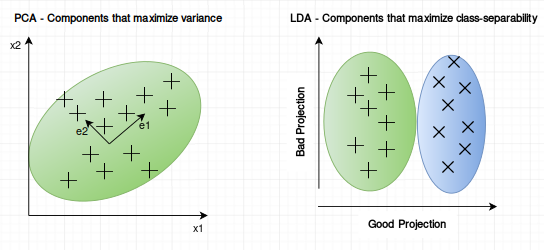
\includegraphics{./Figures/ML/pca_lda}
%      }
% 	\caption[PCA vs LDA]{PCA (left) vs LDA (right)}
% 	\label{fig:pca_lda}
% \end{figure}
\end{itemize}
\subsection{Learning Methods}

After every preprocessing and feature engineering step is completed, comes the learning phase where a set of examples are shown to the classifier, including class labels (supervised learning) or excluding them (unsupervised learning), and the learning process starts. As a result, the classifier is then able to categorize, with a certain accuracy, new unseen data. Some techniques are described bellow:
\begin{itemize}
  \item \textbf{Minimum Distance Classifier} - Minimum Distance Classifiers are template matching system where unseen feature vectors are matched against template prototypes (vectors) representing the classes. This matching usually involves computing the  matching error between both feature vectors using for example the euclidean distance as the error metric. This matching distance can simply be stated as :
  
  \[  \left\Vert  x - m_k \right\Vert \]
 where $x$ is the unseen feature vector and $m_k$ is the feature prototype for class $k$, usually consisting in a feature vector with feature mean values obtained during the training phase. After $k$ tests are performed, the class belonging to the prototype with the minimum distance is chosen. 
  
\item \textbf{k-Nearest Neighbor (kNN)}  - The kNN is a simple and fast unsupervised algorithm that classifies unknown instances based on the majority class from $k$ neighbors. This method starts by constructing a distance matrix between the training samples and the new test sample and chooses the nearest $k$ neighbors. Afterwards, the majority label from these neighbors is assigned to the new data. For two-class problems, $k$ is usually an odd number to prevent ties.

\item \textbf{Naive Bayes} - The Naive Bayes Classifier is a simple supervised probabilistic model based on the Bayes' theorem. The posterior probabilities are computed for each class $wj$ and the class with largest outcome is chosen to classify the feature vector $x$. To achieve this result, the likelihood, prior and evidence probabilities must be calculated, as shown below: 
\[  \text{posterior probability} = \frac{ \text{likelihood}  \cdot \text{prior probability}}{\text{evidence}} \]

\[ P(\omega_j|x) = \frac{p(x|\omega_j) \cdot P(\omega_j)}{p(x)} \]

The main difficulty is to compute the likelihoods $p(x|\omega_j)$ since the other factors are obtained from the data. $P(\omega_j)$ are the prior probabilities and $p(x)$ is a normalization factor which is sometimes omitted. Assuming independence of the features, the likelihoods can obtained as shown bellow:

\[ P(x|\omega_j) = \prod_{k=1}^{d} P(x_k|\omega_j) \]

This simplification allows to compute the class conditional probabilities for each feature separately, reducing complexity and computational costs. 

\item \textbf{Support Vector Machines (SVM)} -  Support vector machines \citep{vapnik1995svm} are optimization methods for binary classification tasks that map the features to a higher dimensional space where an optimal linear hyperplane that separates the existing classes exists. The decision boundary is chosen with the help of some training examples, called the support vectors, that have the widest separation between them and help maximizing the margin between the boundaries of the different classes. The decision surface is in the ``middle'' of these vectors. 
During the training phase, the coefficient vector $w$ and the constant $b$ that define the separating hyperplane are searched such that the following error function is minimized: 

\[ minimize \quad \frac{1}{2} \left \| w \right \|^{2} + C  \sum_{i}^{N} \xi_i \quad s.t  \quad y_i(w \cdot \phi (x_i) + b) \geq 1 - \xi_i  ,\quad \forall x_i \]

where $C$ is an arbitrary constant and $\xi$ are slack variables used to penalize misclassified instances that increase with the distance from the margin. If $C$ is large, the penalty for misclassification is greater. The vectors $x_i$ are the training instances. This method makes use of a kernel function $\phi$ used to transform the input vectors into higher dimensional vectors. New instances are then classified according to which "side" of the hyperplane they are located.

\item \textbf{Decision Tree} - Decision Trees are supervised methods that learn rules based on the training data to classify new instances. The built trees are simple to understand and visualize. During training, each node of the tree is recursively split by the feature that provides, for example, the best information gain.  

\item \textbf{Random Forest} - Random forests ares ensemble methods, i.e., they take into consideration the prediction of several classifiers in order to improve the accuracy and robustness of the prediction results. In the case of random forests, they train a set of random trees with bootstrapped samples (samples drawn with replacement) from the original training data. Each tree is grown by selecting $m$ random features  from the $d$ features and recursively splitting the data by the best splits. The classification of new data is achieved by a majority vote.
\end{itemize}

Each classifier has its own advantages and disadvantages and the right technique should be chosen according to the requirements of the problem-at-hand.
\subsection{Evaluation Metrics}

Experimental evaluation is an important step to assess the effectiveness of a classifier, i.e, the quality of the decisions made by a predictive model on unseen data. In classification tasks, predictions made by a classifier are either considered Positive or False (under some category) and the expected judgments are called True or False (again, under a certain category). Common metrics are \citep{Sebastiani2002MLTC}:

\begin{itemize}
		\item \textbf{Accuracy} - This measure provides a proportion of correctly classified  instances and correctly rejected instances (True Positives and True Negatives) among the whole dataset.
	\begin{figure}[H]
      \centering
    	\[ Acc = \frac{TP + TN}{TP + TN + FP + FN} \]
		\begin{tabular}{lll}
        Acc = Accuracy & TP = True Positives & TN = True Negatives \\ 
        FP = False Positives & FN = False Negatives &
      \end{tabular}
      \end{figure}
      
	\item \textbf{Precision} - This measure provides a proportion of correctly classified  instances (True Positives) among all the positive identified instances (True Positives and False Positives).
	\begin{figure}[H]
      \centering
    	\[ P_i = \frac{TP_i}{TP_i+FP_i} \]
		\begin{tabular}{ll}
        P$_i$ = Precision under Category \textit{i} & TP$_i$ = True Positives under Category \textit{i} \\
        FP$_i$ = False Positives under Category \textit{i} & 
      \end{tabular}
      \end{figure}

    \item \textbf{Recall} - This measure, sometimes called sensitivity, provides a proportion of correctly classified instances (True Positives) among the positive instances that were and should have been correctly identified, i.e., the whole positive part of the dataset (True Positives and False Negatives).\\
      \begin{figure}[H]
      \centering
    	\[ R_i = \frac{TP_i}{TP_i+FN_i} \]
      	\begin{tabular}{ll}
        R$_i$ = Recall under Category \textit{i} & TP$_i$ = True Positives under Category \textit{i} \\
        FN$_i$ = False Negatives under Category \textit{i} & 
      \end{tabular}
      \end{figure}

    \item \textbf{F-measure} - This measure combines precision and recall and provides a balance between them. It is computed as the harmonic mean between the two metrics providing the same weight for both.\\
    \begin{figure}[H]
     \centering
      \[ F_1 = \frac{2 \times P_i \times  R_i}{P_i+R_i} \]
     \begin{tabular}{ll}
        F$_1$ = Harmonic  Mean & P$_i$ = Precision under Category \textit{i} \\
        R$_i$ = Recall under Category \textit{i} & 
     \end{tabular}
     \end{figure}
\end{itemize}

These metrics provides insights on how the model behaves. We can go further and compute the previous estimations in different ways such as:
\begin{itemize}
	\item \textbf{Micro Averaging} - In this case the entire text is treated as a single document and the individual correct classifications are summed up.	\\
    \begin{figure}[H]
      \centering
      \[ P^{\mu} = \frac{\sum_{i=1}^{|C|} TP_i}{\sum_{i=1}^{|C|} TP_i + FP_i} \]
      \begin{tabular}{ll}
        P$^{\mu}$ = Micro Precision, & C = Set of Classes\\
        TP = True Positives, & FP = False Positives
      \end{tabular}
	\end{figure}
    
     \begin{figure}[H]
      \centering
      \[ R^{\mu} = \frac{\sum_{i=1}^{|C|} TP_i}{\sum_{i=1}^{|C|} TP_i + FN_i} \]
      \begin{tabular}{ll}
        R$^{\mu}$ = Micro Recall, & C = Set of Classes\\
        TP = True Positives, & FN = False Negatives
      \end{tabular}
	\end{figure}
    \item \textbf{Macro Averaging} - In this case the precision and recall metrics are computed for each document and then averaged.\\    	
	
	\begin{figure}[H]
      \centering
      \[ P^{M} = \frac{\sum_{i=1}^{|C|} P_i}{|C|} \]
      \begin{tabular}{ll}
        $P^{M}$ = Macro Precision, & C = Set of Classes\\
      \end{tabular}
	\end{figure}
    
    \begin{figure}[H]
      \centering
      \[ R^{M} = \frac{\sum_{i=1}^{|C|} R_i}{|C|} \]
      \begin{tabular}{ll}
        R$^{M}$ = Macro Recall, & C = Set of Classes\\
      \end{tabular}
	\end{figure}
\end{itemize}

In addition to the previous averages, the standard deviation is a common dispersion metric that may be computed as follows:
    \begin{figure}[H]
      \centering
\begin{tabular}{ll}
		\Large
		\( \sigma = \frac{1}{N-1}\sum_{i=1}^{|N|}{(x_i - \bar{x})^2} \) & \\
		\\
        N = Number of samples, & x$_i$ = Result of the i-th measurement \\
		$\bar{x}$ = Arithmetic mean of the N results
      \end{tabular}
\end{figure}

These evaluation methods can give different results. Macro averaging gives equal weights for each class, even if there are unbalanced classes. On the other hand, micro averaging gives equal weight to the documents under evaluation, but it can happen that large classes dominate smaller classes. Therefore, macro averaging provides a sense of effectiveness on small classes, increasing their importance. Usually, the choice of which method to use depends on the requirements of the application.

\begin{itemize}
\item \textbf{Receiver Operating Characteristics (ROC)} - ROC curves \citep{Fawcett2006ROC} are useful graphs to visualize the performance of binary classifiers. They are useful to compare the rates at which the classifier is making correct predictions (True Positive Rate plotted on the Y axis) against the rate of false alarms (False Positive Rate plotted on the X axis). Important points in this graph are the lower left point (0,0), representing a classifier that never classify positive instances, neither having False Positives or True Positives. On the other hand, the upper right point (1,1) represents a classifier that classifies every instance as positive, disregarding if it is a false positive or not. Finally, the point (0,1) represents the perfect classifier, where every instance was correctly classified. Figure \ref{fig:roc} illustrates this idea, showing three hypothetical classifiers and the regions of good and poor performance, which are above or below the line defined by a random classifier making correct random guesses half of the time.  The area bellow the ROC curve is called Area Under the Curve (AUC) and is also a good measure. A perfect classifier would have an AUC of 1.0 while a random classifier would only have 0.5.

\begin{figure}[htp]
	\centering
	\resizebox{\textwidth}{!}{
  	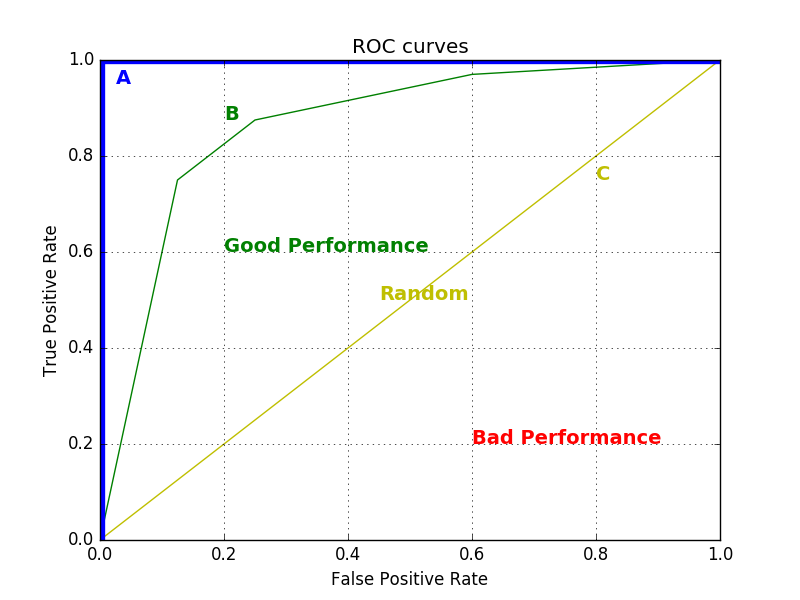
\includegraphics{./Figures/ML/roc}
     }
	\caption[ROC curves of 3 hypothetical classifiers]{ROC curves of 3 hypothetical classifiers: Perfect (A), good (B) and random (C)}
	\label{fig:roc}
\end{figure}

\item \textbf{Precision-Recall Curves (PR)} - The Precision-Recall Curve plots the trade-off between the precision and recall achieved by a classifier, by showing the recall on the X axis and precision on the Y axis. An important point in this graph is the upper right point (1,1) which represents the ideal classifier having maximum precision and recall. Figure \ref{fig:pr} shows three hypothetical classifiers and the areas of good and bad performance, which are above or below the line defined by a random classifier. The area bellow the PR curve is called Average Precision (AP) and is also a good measure. A perfect classifier would have an Average Precision of 1.0 while a random classifier would only have 0.5. 

\begin{figure}[htp]
	\centering
	\resizebox{\textwidth}{!}{
  	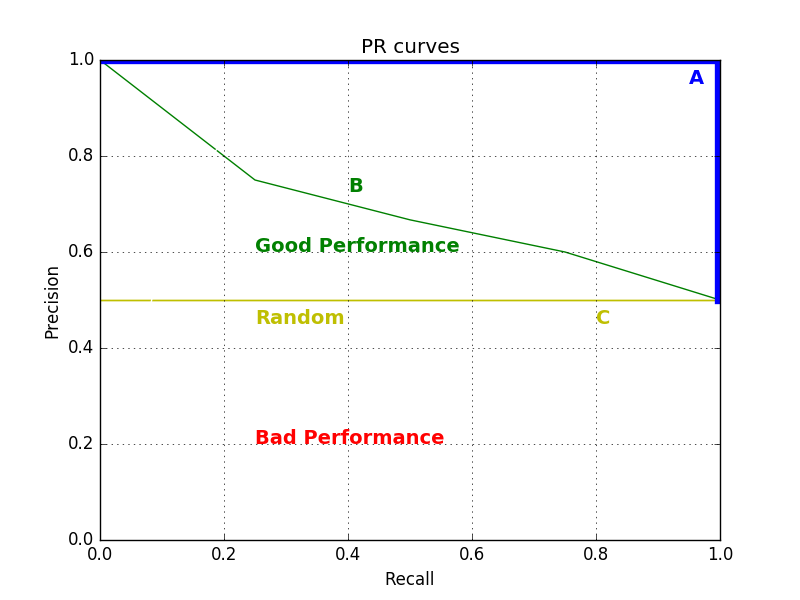
\includegraphics{./Figures/ML/pr}
     }
	\caption[Precision-Recall curves of 3 hypothetical classifiers]{Precision-Recall curves of 3 hypothetical classifiers: Perfect (A), good (B) and random (C)}
	\label{fig:pr}
\end{figure}

\item \textbf{Stratified K-fold Cross Validation} - A popular technique to evaluate the performance of the system is to split the data into training and testing sets, using the later to estimate the true generalization performance of the classifier. However, this may bring some issues such as the trade-offs between the percentage splits or the representativity of the test set \citep{Polikar2006PR}. A popular accepted approach is to split the entire dataset into $k$ representative partitions, using $k-1$ of these partitions for training and the remaining one for testing. This process is then repeated $k$ times, (each time using a different test partition) and the results averaged. 
\end{itemize}

% https://gate.ac.uk/sale/tao/splitch10.html#x14-26300010
% https://gate.ac.uk/sale/tao/splitch19.html#x24-45300019.1
% http://www.cse.unsw.edu.au/~billw/mldict.html
% http://nlp.stanford.edu/IR-book/html/htmledition/text-classification-and-naive-bayes-1.html
% http://arxiv.org/pdf/cs/0110053.pdf
% http://www.aaai.org/ojs/index.php/aimagazine/article/view/406/342


\section{Relation to this work}

In this chapter we started by defining some classical notions about relevance and how it is a concept well studied in academic disciplines such as Information Retrieval. However, it should be noted that these classical views are not aligned with the approach of this work. Instead, we explore another direction by defining relevance in terms of journalistic criteria, such as: controversialness, interestingness, meaningfulness, novelty, reliability and scope. According to the relation between the previous attributes, a document should be classified as relevant or irrelevant. Likewise, we can treat these attributes as their own sub-problems. \\
The presented NLP tasks are also a crucial part of this work, since they provide the features to be used in the classification experiments. Since the type of our study object is raw text, the NLP field comes as a natural choice in tackling the problem of feature extraction. \\
We also reviewed some important pattern recognition concepts. First, we define our task as a binary problem, which has to classify text documents as either relevant or irrelevant. It is important to note that mentioned sub-problems are also binary problems by themselves, meaning that a document can be classified as controversial or not uncontroversial, interesting or uninteresting, meaningful or meaningless, new or old, reliable or unreliable and finally wide or narrow. Since we are dealing with text, a common problem is the high dimensionality of the feature space. Therefore, we may use well known techniques to reduce the problem to its most important, informative and discriminatory attributes. Finally, we use learning and evaluation methods to build and evaluate the accuracy our models.

Table \ref{tab:methods-used} summarizes this view by presenting the used journalistic relevance criteria, the used natural language processing tasks and machine learning methods used. 


\begin{table}[H]
\centering
\resizebox{\textwidth}{!}{%
\begin{tabular}{c|c|ccccc}
\hline
\multicolumn{1}{|c|}{\textbf{Definition  of Relevance}} & \textbf{NLP Tasks} & \multicolumn{5}{c|}{\textbf{Machine Learning Methods}} \\ \hline
\multicolumn{1}{|c|}{\textbf{Criteria}} & \textbf{Extraction} & \multicolumn{1}{c|}{\textbf{Preprocessing}} & \multicolumn{1}{c|}{\textbf{Selection}} & \multicolumn{1}{c|}{\textbf{Reduction}} & \multicolumn{1}{c|}{\textbf{Models}} & \multicolumn{1}{c|}{\textbf{Evaluation}} \\ \hline
\multicolumn{1}{|c|}{Controversialness} & Part-of-Speech & \multicolumn{1}{c|}{Standardization} & \multicolumn{1}{c|}{Info. Gain} & \multicolumn{1}{c|}{PCA} & \multicolumn{1}{c|}{MDC} & \multicolumn{1}{c|}{Accuracy} \\ \hline
\multicolumn{1}{|c|}{Informativeness} & Chunking & \multicolumn{1}{c|}{Normalization} & \multicolumn{1}{c|}{Gain Ratio} & \multicolumn{1}{c|}{} & \multicolumn{1}{c|}{kNN} & \multicolumn{1}{c|}{Precision} \\ \cline{1-4} \cline{6-7} 
\multicolumn{1}{|c|}{Meaningfulness} & Named Entities & \multicolumn{1}{c|}{Scaling} & \multicolumn{1}{c|}{Fisher} & \multicolumn{1}{c|}{} & \multicolumn{1}{c|}{NB} & \multicolumn{1}{c|}{Recall} \\ \cline{1-4} \cline{6-7} 
\multicolumn{1}{|c|}{Novelty} & Polarity of words & \multicolumn{1}{c|}{} & \multicolumn{1}{c|}{Pearson} & \multicolumn{1}{c|}{} & \multicolumn{1}{c|}{SVM} & \multicolumn{1}{c|}{F$_1$} \\ \cline{1-2} \cline{4-4} \cline{6-7} 
\multicolumn{1}{|c|}{Reliability} & LDA topics & \multicolumn{1}{c|}{} & \multicolumn{1}{c|}{Chi-square} & \multicolumn{1}{c|}{} & \multicolumn{1}{c|}{DT} & \multicolumn{1}{c|}{ROC} \\ \cline{1-2} \cline{4-4} \cline{6-7} 
\multicolumn{1}{|c|}{Scope} & N-gram &  &  & \multicolumn{1}{c|}{} & \multicolumn{1}{c|}{RF} & \multicolumn{1}{c|}{AP} \\ \cline{1-2} \cline{6-7} 
 & Stemming &  &  &  & \multicolumn{1}{c|}{} & \multicolumn{1}{c|}{k-Fold-CV} \\ \cline{2-2} \cline{7-7} 
 & Lemmatization &  &  &  &  &  \\ \cline{2-2}
\end{tabular}%
}
\caption[Methods used in this work]{Methods used in this work}
\label{tab:methods-used}
\end{table}




%----------------------------------------------------------------------------------------

%----------------------------------------------------------------------------------------





